\chapter{Technical Specification}
\section{Protocol}

In this section, we provide an explanation of the protocol and the values used in it.

The protocol of our signing service consists of five main phases:

\begin{itemize}
	\item Pre-Login (see~\ref{subsec:pre-login})
	\item Login (see~\ref{subsec:login})
	\item Post-Login (see~\ref{subsec:post-login})
	\item Signature Generation (see~\ref{subsec:signature-generation})
	\item Signature Verification (see~\ref{subsec:signature-verification})
\end{itemize}

For a high-level overview of these phases, see figure~\ref{fig:highlevelprotocoloverview}.

\begin{figure}
	\begin{center}
		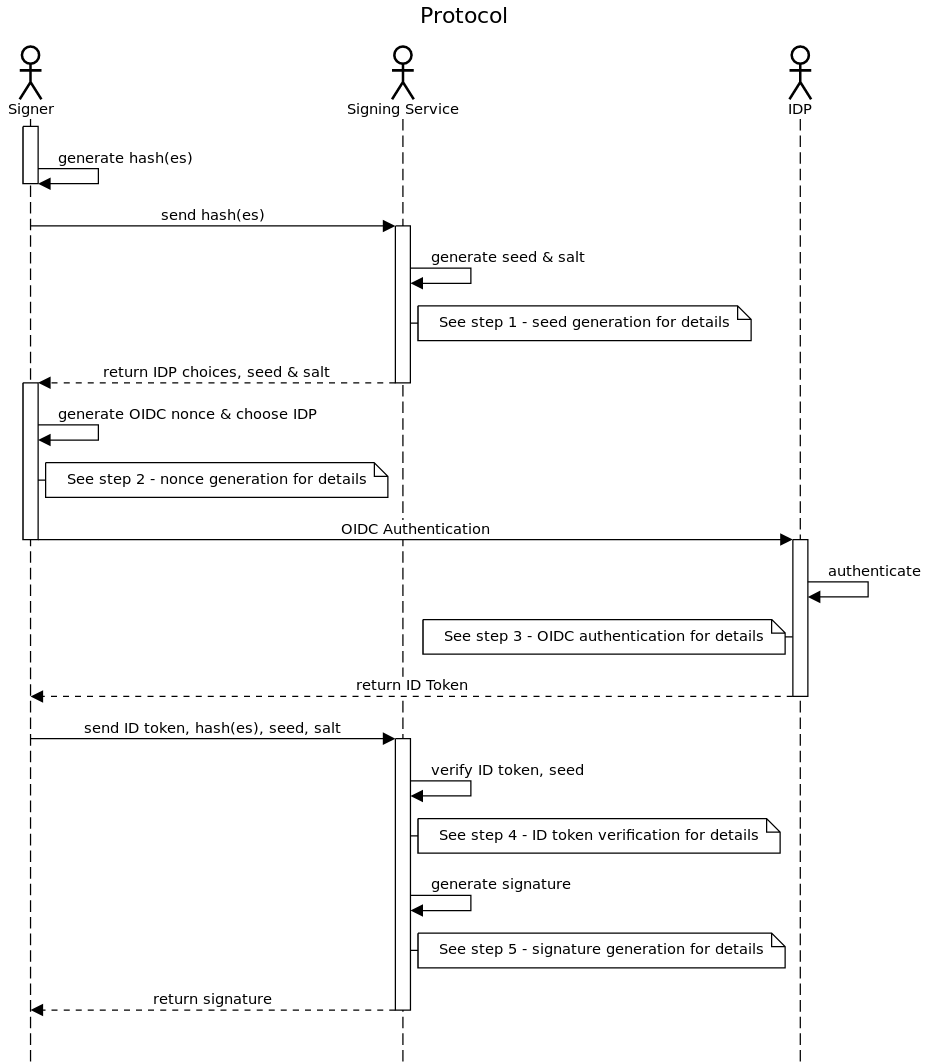
\includegraphics[scale=0.5]{images/protocol_signature_generation_high_level.png}
		\caption{High-level protocol overview}
		\label{fig:highlevelprotocoloverview}
	\end{center}
\end{figure}

\subsection{Pre-Login}\label{subsec:pre-login}
In this phase the signer provides a list of hashes to signing service
(this list may consist of just one entry in case the signer wishes to sign a single document).

Then, the signing service generates a random \texttt{seed} value.
This \texttt{seed}, together with a \texttt{secret} known to the server only,
is be used to calculate the key that is used to generate a \gls{HMAC} of the sorted list of hashes.
The resulting \gls{HMAC} is used as a \texttt{salt} for the hashes in the \gls{OIDC} nonce.
The key consists of the \texttt{secret} appended to the \texttt{seed}.

\paragraph{Purpose of the salt}
The salt is used to mask the document hashes in the \gls{OIDC} nonce both from the \gls{IDP},
so that it doesn't know whether two people sign the same document(s),
and the recipient of the signature, as they need a list of all hashes that have been signed together
in order to be able to verify the signature.

\paragraph{Purpose of the seed}
The \texttt{seed} is used as a \gls{CSRF} protection mechanism without the need for the server to keep any state.
If no such \texttt{seed} were used for generating the salt,
the signing server would be required to keep it in memory and attach it to the users session,
in order to be able to verify whether the hashes or the salt weren't replaced while generating the \gls{OIDC} nonce
(thus establishing the secure link between the document hashes and the authentication).
If the signing server didn't verify this, it would enable attackers to skip the Pre-Login step (see~\ref{subsec:pre-login}).

The server than returns a list of \gls{IDP} choices as well as the \texttt{seed} and the \texttt{salt} to the client.

For a sequence diagram of this phase, see figure~\ref{fig:seedgenerationstep}.

\begin{figure}
	\begin{center}
		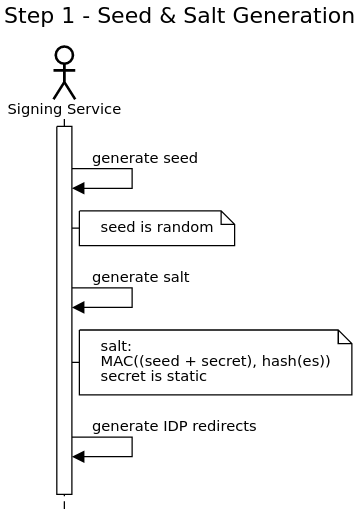
\includegraphics[scale=0.5]{images/protocol_step1_seed_generation.png}
		\caption{Seed generation step}
		\label{fig:seedgenerationstep}
	\end{center}
\end{figure}

\subsection{Login}\label{subsec:login}
The client generates the nonce used for the \gls{OIDC} request,
consisting of the hash of the sorted list of \gls{HMAC}s of the hashes with the \texttt{salt} as key.
For a graphical representation of this, see figure~\ref{fig:noncegenerationstep}.
Next, the client chooses an \gls{IDP}, and adds the nonce they just generated to the request parameters and then follows the link.
The client then authenticates with the \gls{IDP} and receives their ID token as seen in figure~\ref{fig:oidcauthenticationstep}.

\begin{figure}
	\begin{center}
		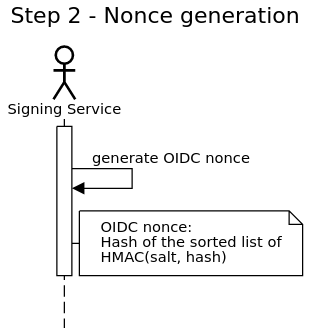
\includegraphics[scale=0.5]{images/protocol_step2_nonce_generation.png}
		\caption{Nonce generation step}
		\label{fig:noncegenerationstep}
	\end{center}
\end{figure}

\begin{figure}
	\begin{center}
		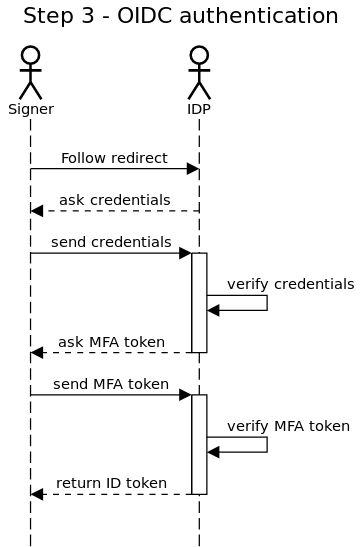
\includegraphics[scale=0.5]{images/protocol_step3_oidc_authentication.png}
		\caption{OIDC authentication step}
		\label{fig:oidcauthenticationstep}
	\end{center}
\end{figure}

\subsection{Post-Login}\label{subsec:post-login}
As shown in figure~\ref{fig:tokenverificationstep},
the client sends the ID token, the list of hashes, the \texttt{seed} and the \texttt{salt} to the signing service.
The signing service then verifies the \texttt{salt}, OIDC nonce and ID token.
After this step, the \texttt{seed} is not used anymore and should be discarded.


\begin{figure}
	\begin{center}
		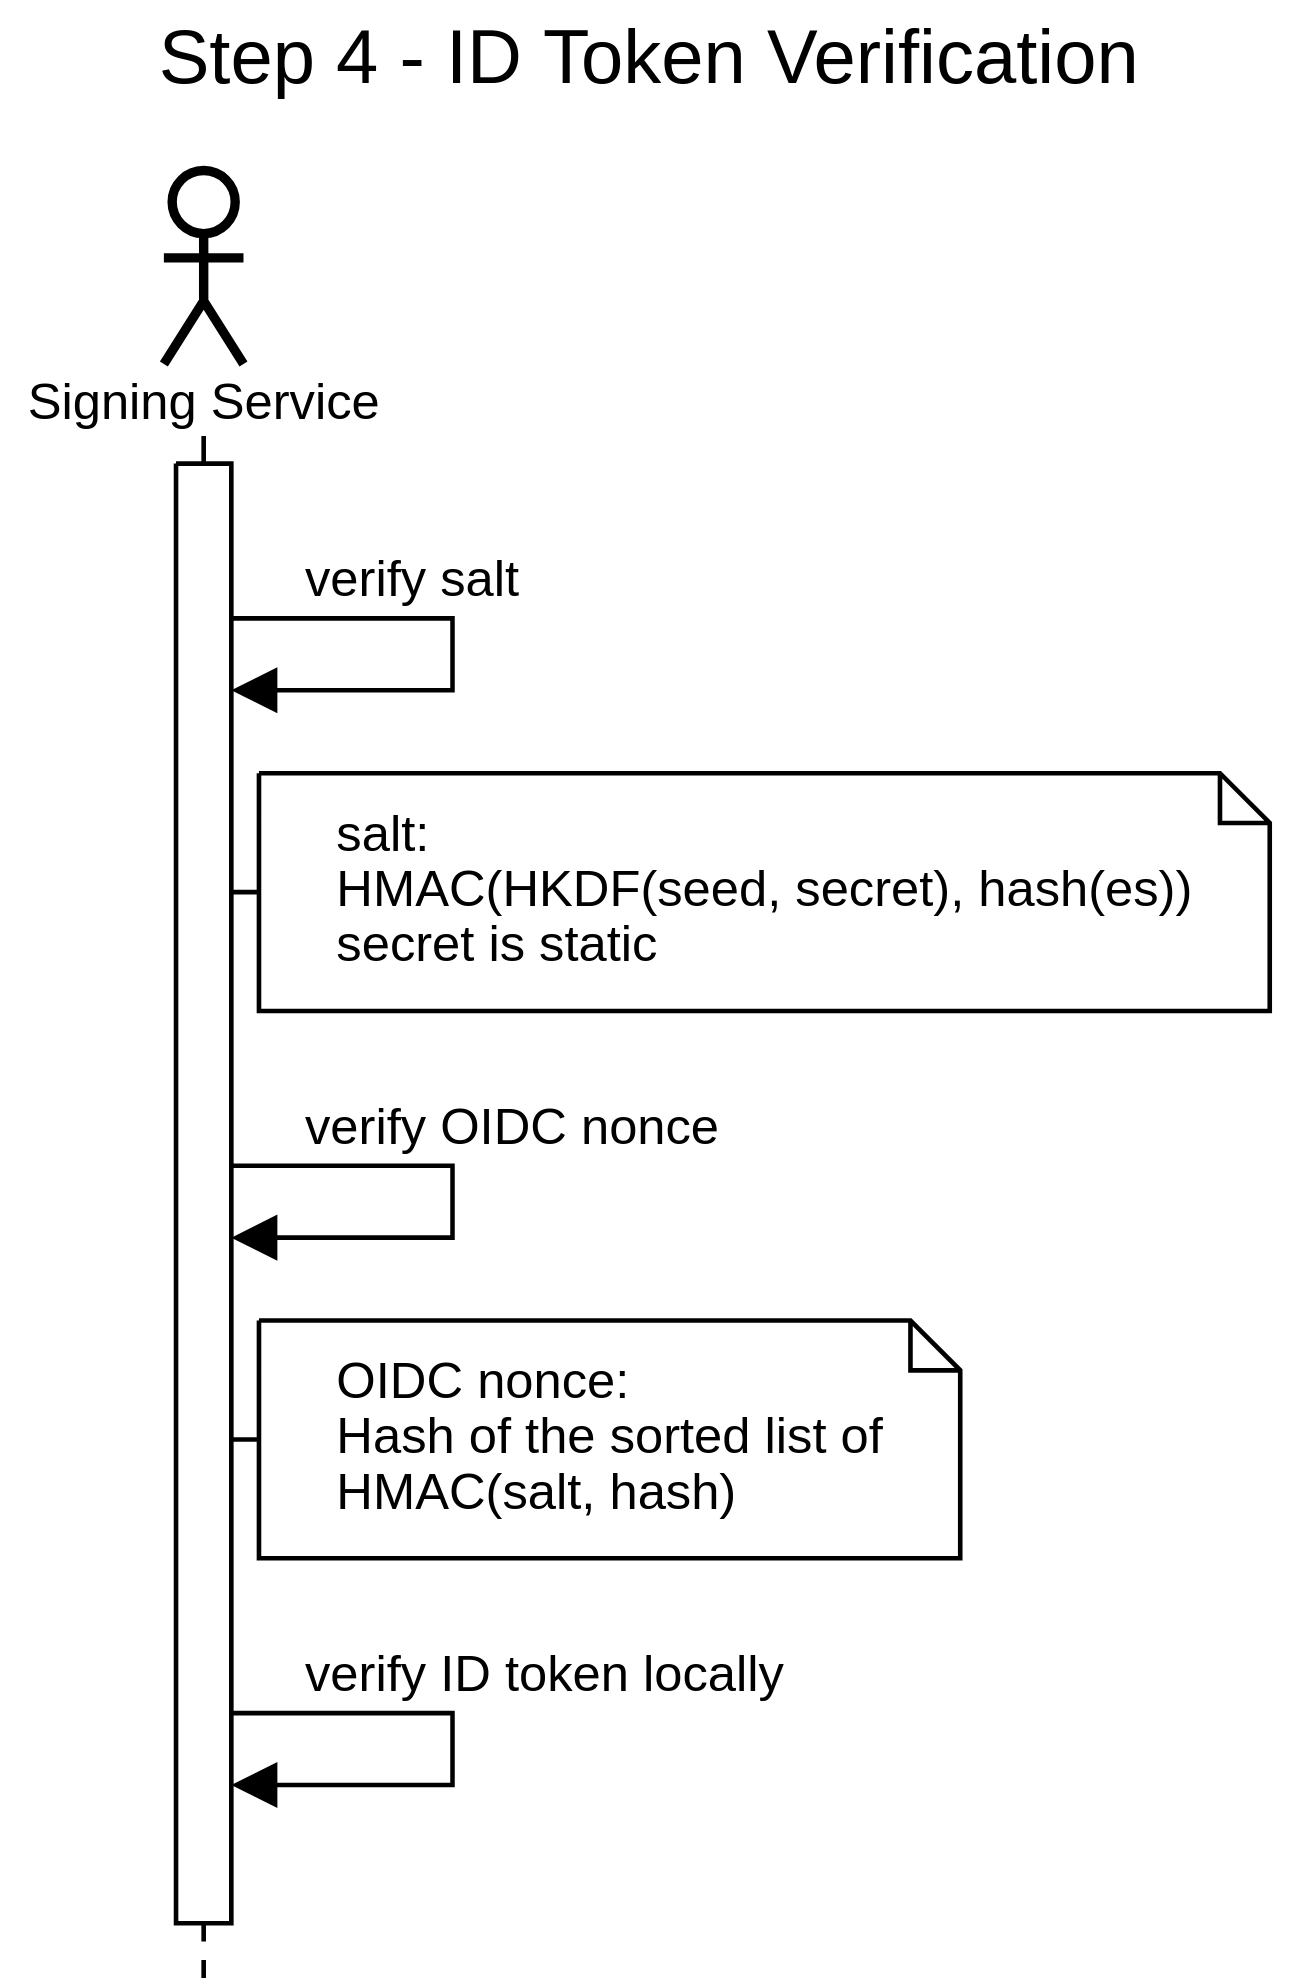
\includegraphics[scale=0.5]{images/protocol_step4_id_token_verification.png}
		\caption{Token verification step}
		\label{fig:tokenverificationstep}
	\end{center}
\end{figure}

\subsection{Signature Generation}\label{subsec:signature-generation}
The signing server requests a new signing key from the \gls{HSM}, which in turn generates a private key and returns a \gls{CSR}.
This \gls{CSR} is sent to the \gls{CA} where it is signed and the signed certificate returned.

Each hash is then submitted to the \gls{HSM} to be signed by the signing key.

Then, for each hash an intermediate signature file consisting of the signed hash,
the ID token, the \texttt{salt} and a sorted list of all other salted hashes is created.
The hash of this file is sent to a \gls{TSA} where a signed timestamp is created and returned.

Finally, the signed timestamp, and all the certificate chains,
\gls{OCSP} responses and \gls{CRL}s of the involved parties,
is added to signature file, which is then returned to the user.

See figure~\ref{fig:signaturegenerationstep} for a sequence diagram of this process.

\begin{figure}
	\begin{center}
		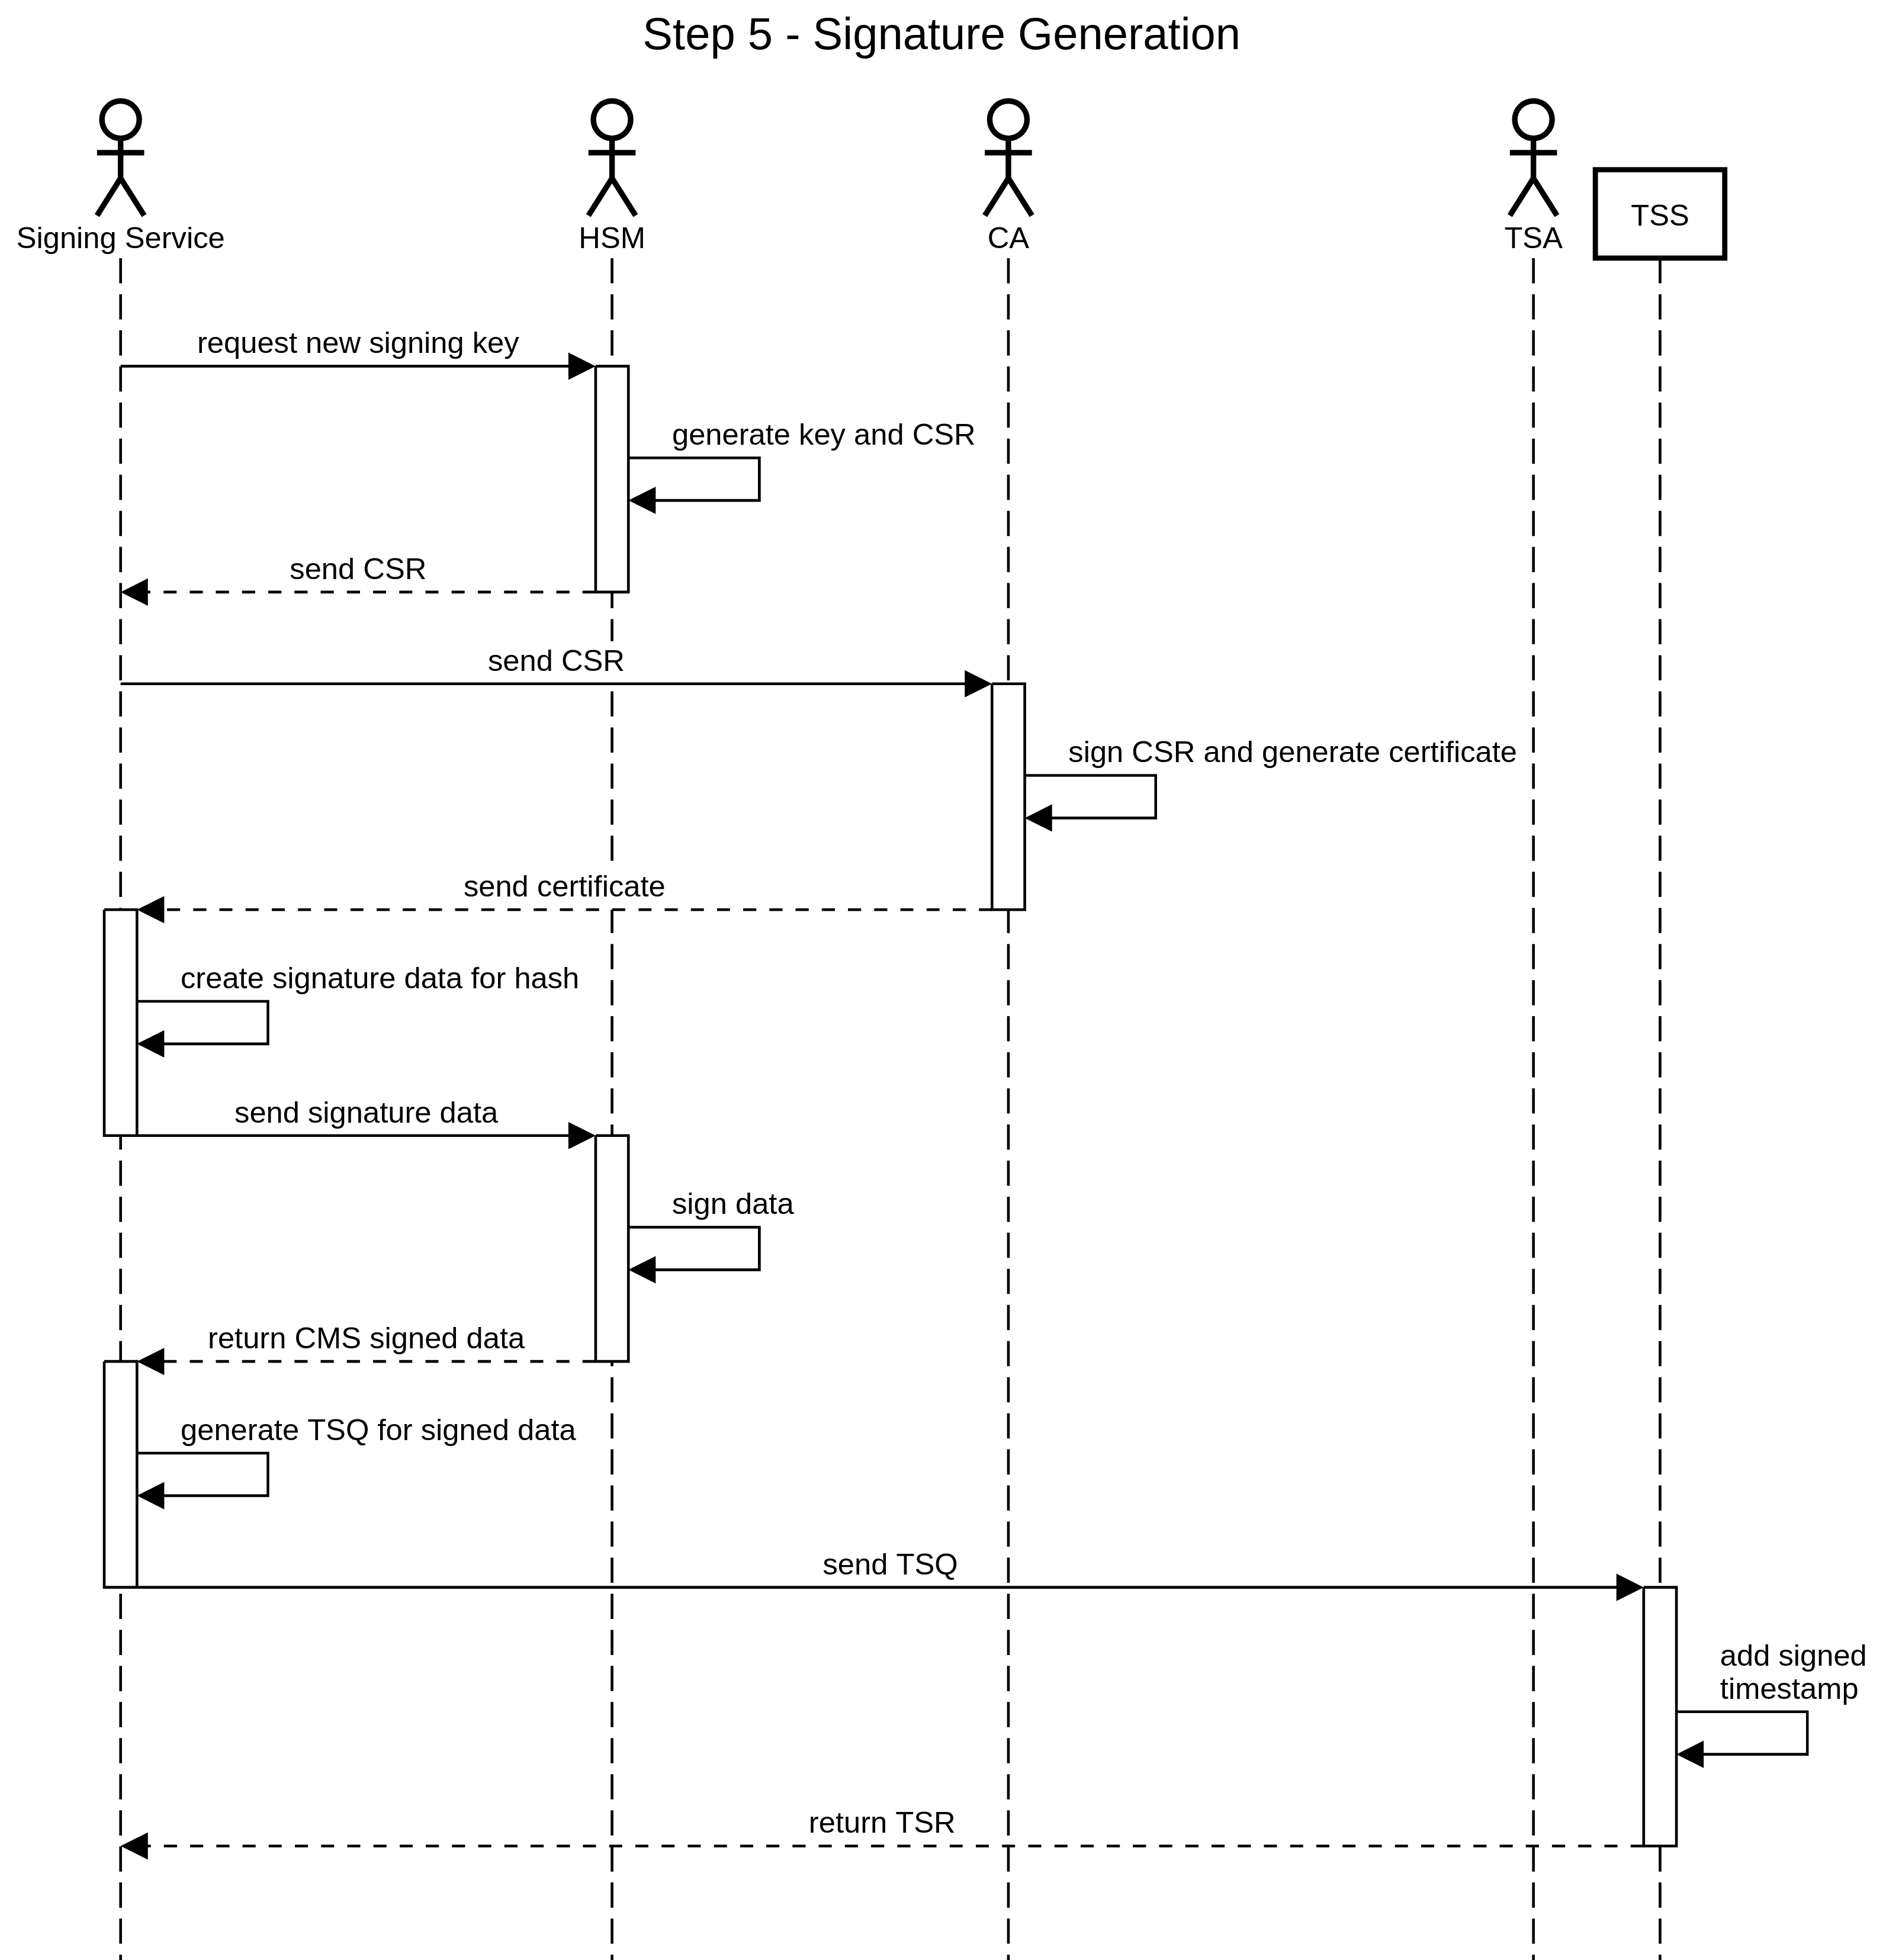
\includegraphics[scale=0.45]{images/protocol_step5_signature_generation.png}
		\caption{Signature generation step}
		\label{fig:signaturegenerationstep}
	\end{center}
\end{figure}

\subsection{Signature Verification}\label{subsec:signature-verification}

The signature verification can either be online (figure~\ref{fig:onlinesignatureverificationprotocol})
or offline (figure~\ref{fig:offlinesignatureverificationprotocol}).

For online verification, the user simply uploads the list of hashes and the signature file to the verification service.

\begin{figure}
	\begin{center}
		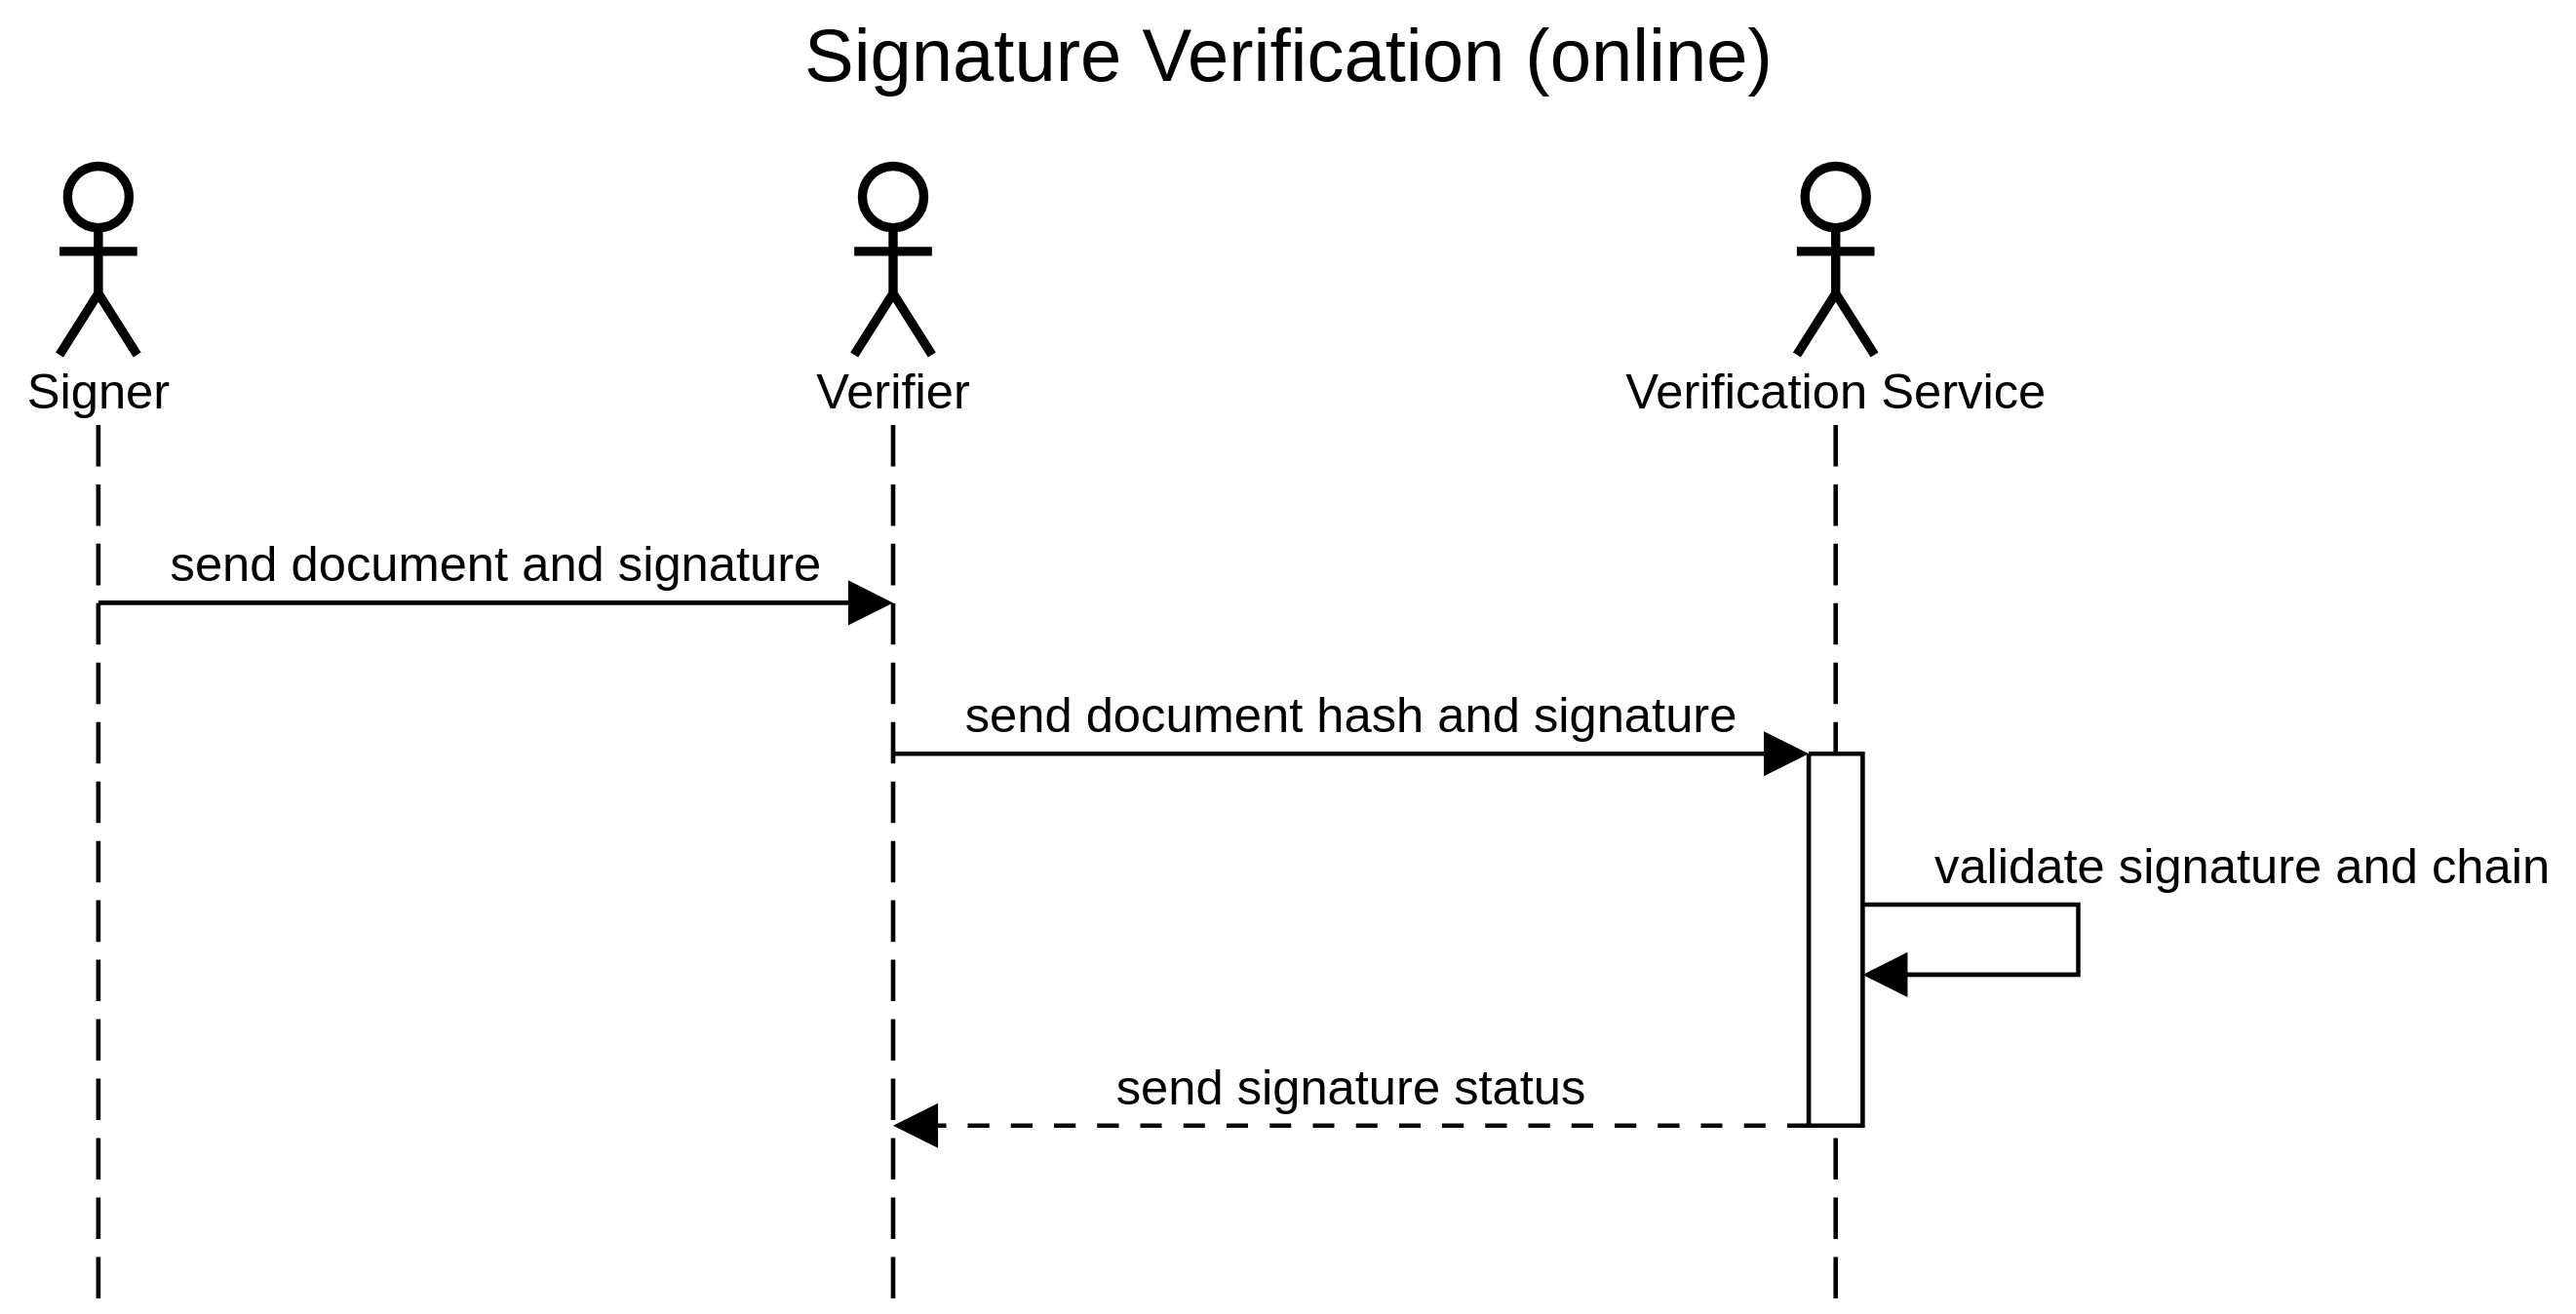
\includegraphics[scale=0.5]{images/protocol_online_verification_high_level.png}
		\caption{Online Signature Verification Protocol}
		\label{fig:onlinesignatureverificationprotocol}
	\end{center}
\end{figure}

For the offline verification, the user downloads the verification programme and starts it.
Then, they upload the list of hashes and signature file just as if they were using online verification,
but to their own copy of the verification service running on their computer without needing any network connection
instead of a remote verification service.

\begin{figure}
	\begin{center}
		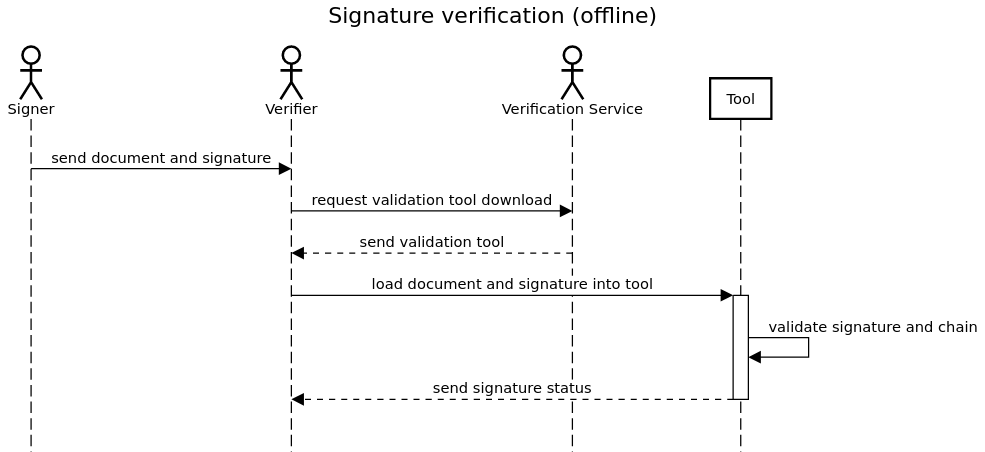
\includegraphics[scale=0.5]{images/protocol_offline_verification_high_level.png}
		\caption{Offline Signature Verification Protocol}
		\label{fig:offlinesignatureverificationprotocol}
	\end{center}
\end{figure}

To verify a signature,
the verifier first needs to verify the chain of signed timestamps and their respective \gls{CA} chains (figure~\ref{fig:timestampverificationstep}).

\begin{figure}
	\begin{center}
		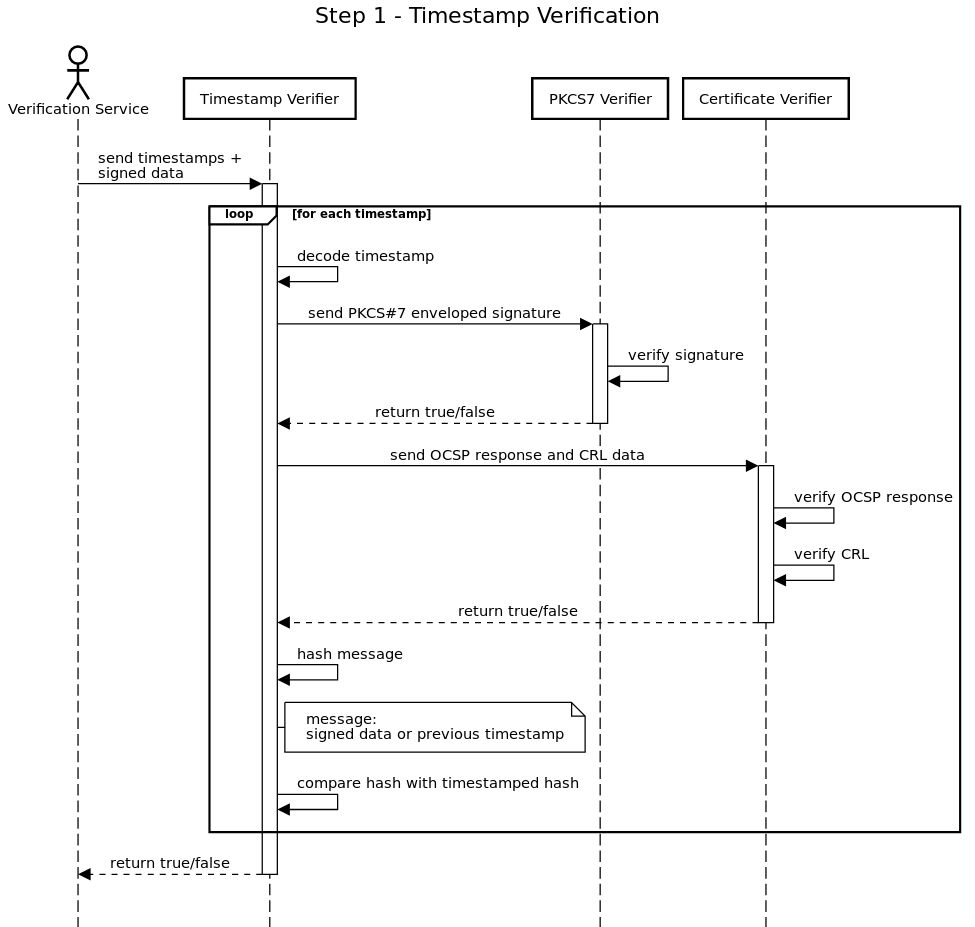
\includegraphics[scale=0.5]{images/protocol_verification_step1_timestamp.png}
		\caption{Timestamp verification step}
		\label{fig:timestampverificationstep}
	\end{center}
\end{figure}

The signature itself can then be verified (figure~\ref{fig:signaturegenerationstep}), along with
the certificate chain for the signing certificate.

\begin{figure}
	\begin{center}
		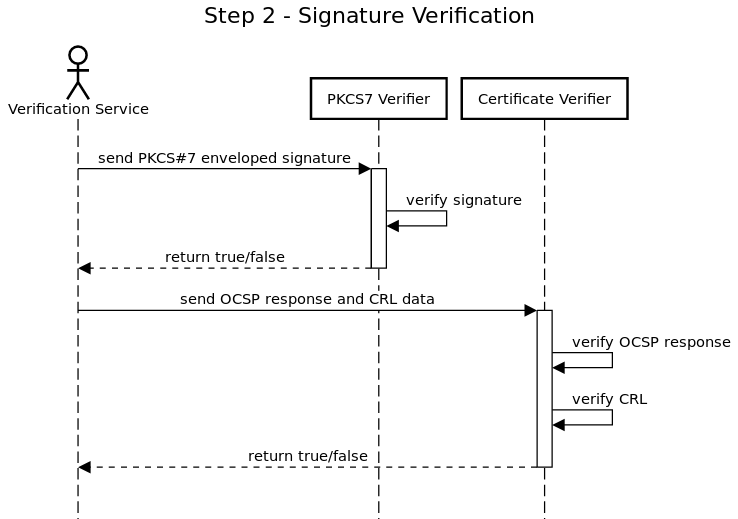
\includegraphics[scale=0.5]{images/protocol_verification_step2_signature.png}
		\caption{Signature verification step}
		\label{fig:signatureverificationstep}
	\end{center}
\end{figure}

Then, the ID token itself needs to be verified,
as well as the certificate chain of the key used to sign the ID token (figure~\ref{fig:idtokenverification}).

\begin{figure}
	\begin{center}
		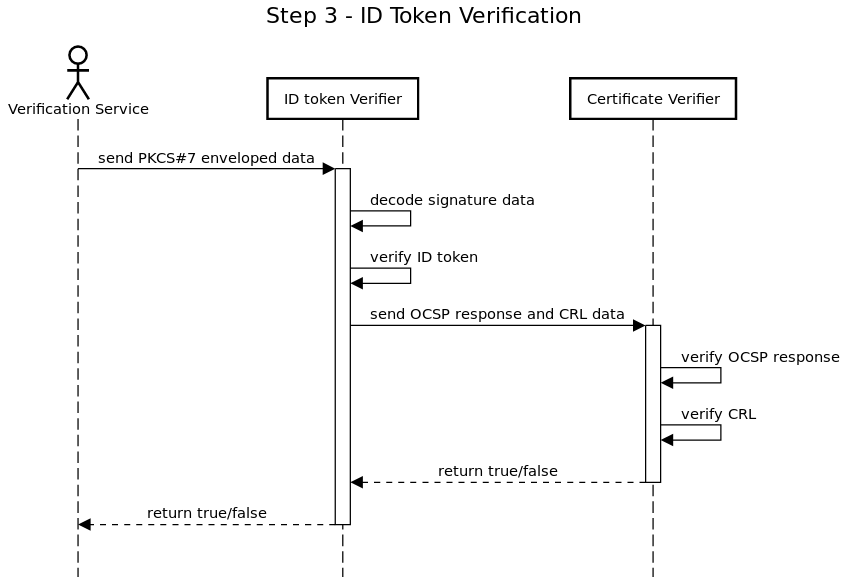
\includegraphics[scale=0.5]{images/protocol_verification_step3_id_token.png}
		\caption{ID token verification}
		\label{fig:idtokenverification}
	\end{center}
\end{figure}

In order to verify the link of the document hashes with the ID token,
the document hash needs to be salted, inserted into the sorted list of the other salted hashes,
and the resulting list hashed again.
The result must be the same as the nonce in the ID token.
At last, the hash of the document must match the included hash.
Figure~\ref{fig:signaturedataverification} illustrates this process.

\begin{figure}
	\begin{center}
		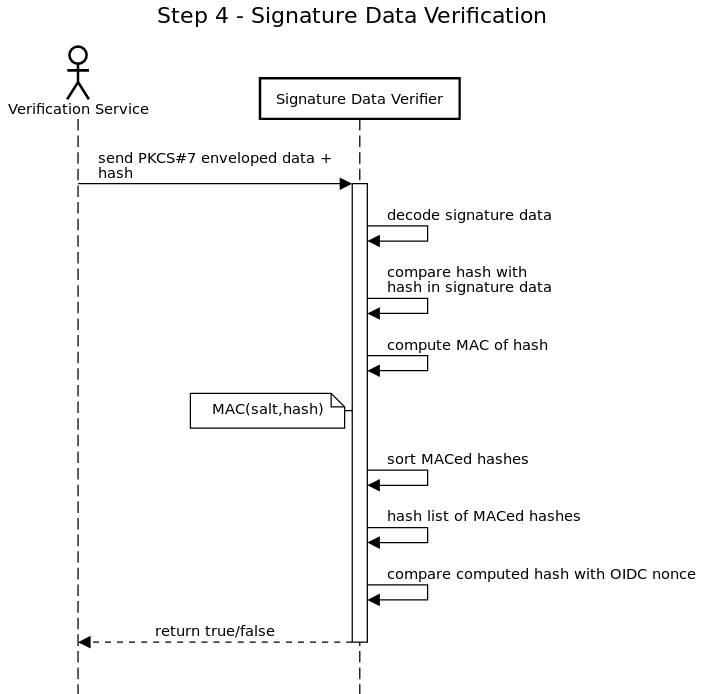
\includegraphics[scale=0.5]{images/protocol_verification_step4_signature_data.png}
		\caption{Signature data verification}
		\label{fig:signaturedataverification}
	\end{center}
\end{figure}

\section{REST API}\label{sec:rest-api}

\subsection{Signing Service}
Endpoints:

\begin{tabular}{|l|l|l|}
	\hline
	Endpoint & Method & Description \\ \hline
	/api/v1/login & POST & send hashes to get oidc providers \\ \hline
	/api/v1/sign & POST & sign hashes \\ \hline
	/api/v1/signatures/:id & GET & retrieve signature \\ \hline
\end{tabular}

\subsubsection{login}
Input:

\begin{tabular}{|l|l|l|l|}
	\hline
	Parameter & Presence & Type & Description \\ \hline
	hashes & MANDATORY & list(string) & Hashes of the documents to be signed \\ \hline
\end{tabular}

Output:

\begin{tabular}{|l|l|l|l|}
	\hline
	Parameter & Presence & Type & Description \\ \hline
	providers & MANDATORY & dictionary[string]url & List of providers with the redirect url \\ \hline
	seed & MANDATORY & string & Seed for generating the salt \\ \hline
	salt & MANDATORY & string & Salt for generating the OIDC nonce \\ \hline
\end{tabular}

Sample Request:
\begin{lstlisting}[caption={login request}, captionpos=b, language=JavaScript, label={lst:hashesrequest}]
POST /api/v1/hashes HTTP/1.1
Host: service.example.org
Content-Type: application/json

{
  "hashes": [
  "e8a96e6203b9c0df058ba862abc63d9c520157faef6d5d54e54e526b0a85b2be",
  "0b9a7fd3e612061a7fe6d834e102a143170f33d0e8c5a8eb79416aa3eb53c0d6"
  ]
}
\end{lstlisting}

Sample Response:
\begin{lstlisting}[caption={login response}, captionpos=b, language=JavaScript, label={lst:hashesresponse}]
HTTP/1.1 201 Created
Content-Type: application/json

{
  "providers": {
  	"SwissID": "https://...&nonce=6cd7ef99e5e79d68d681e5d097b7f805381c4d013152fa3f26d06bd728ae49fa",
	"Google": "https://...&nonce=6cd7ef99e5e79d68d681e5d097b7f805381c4d013152fa3f26d06bd728ae49fa"
  },
  "seed": "84c97acc49335faa0266fb29b4228205e9400a85a10faa68ec30cf894e1730ed",
  "salt": "cfb663431af5e2d68be48867f93e86e477cd7eeefc10b16a51c238d2c810561b"
}
\end{lstlisting}

\subsubsection{sign}
Input:

\begin{tabular}{|l|l|l|l|}
	\hline
	Parameter & Presence & Type & Description \\ \hline
	id\_token & MANDATORY & string & OIDC ID token \\ \hline
	seed & MANDATORY & string & Seed for generating the salt \\ \hline
	salt & MANDATORY & string & Salt for generating the OIDC nonce \\ \hline
	hashes & MANDATORY & list(string) & Hashes of the documents to be signed \\ \hline
\end{tabular}

Output:

\begin{tabular}{|l|l|l|l|}
	\hline
	Parameter & Presence & Type & Description \\ \hline
	signature urls & MANDATORY & dictionary[string]url & List of urls to the generated signature files for each hash\\ \hline
\end{tabular}

Sample Request:
\begin{lstlisting}[caption={sign request}, captionpos=b, language=JavaScript, label={lst:signrequest}]
POST /api/v1/sign HTTP/1.1
Host: service.example.org
Content-Type: application/json

{
  "idtoken": {...},
  "seed": "84c97acc49335faa0266fb29b4228205e9400a85a10faa68ec30cf894e1730ed",
  "salt": "cfb663431af5e2d68be48867f93e86e477cd7eeefc10b16a51c238d2c810561b",
  "hashes": [
    "e8a96e6203b9c0df058ba862abc63d9c520157faef6d5d54e54e526b0a85b2be",
    "0b9a7fd3e612061a7fe6d834e102a143170f33d0e8c5a8eb79416aa3eb53c0d6"
  ]
}
\end{lstlisting}

Sample Response:

\begin{lstlisting}[caption={sign response}, captionpos=b, language=JavaScript, label={lst:signresponse}]
HTTP/1.1 201 Created
Content-Type: application/json

{
	"signatures": {
		"e8a96e6203b9c0df058ba862abc63d9c520157faef6d5d54e54e526b0a85b2be": "https://signingservice.local/api/v1/signatures/64ba127f549d9b480c1e2a304da1f7f7787cdcaed64a57b7a1ec9773c0246da1",
		"0b9a7fd3e612061a7fe6d834e102a143170f33d0e8c5a8eb79416aa3eb53c0d6": "https://signingservice.local/api/v1/signatures/0b1131c417cafcc5a5f259d357903026f8e0c4f85e3ca0b68f3d55b8e32a55e8"
	}
}
\end{lstlisting}

\subsubsection{signatures/:id}
Input:

\begin{tabular}{|l|l|l|l|}
	\hline
	Parameter & Presence & Type & Description \\ \hline
	id & MANDATORY & string & id of the hash that was signed \\ \hline
\end{tabular}

Output:

\begin{tabular}{|l|l|l|l|}
	\hline
	Parameter & Presence & Type & Description \\ \hline
	signature & MANDATORY & binary & base64 encoded signature for the requested hash \\ \hline
\end{tabular}

Sample Request:

\begin{lstlisting}[caption={signature request}, captionpos=b, language=JavaScript, label={lst:signaturerequest}]
GET /api/v1/signatures/e8a96e6203b9c0df058ba862abc63d9c520157faef6d5d54e54e526b0a85b2be HTTP/1.1
Host: service.example.org
Content-Type: application/json
\end{lstlisting}

Sample Response:

\begin{lstlisting}[caption={signature response}, captionpos=b, language=JavaScript, label={lst:signatureresponse}]
HTTP/1.1 200 OK
Content-Type: application/json

{
  "signature": "IyMjIFJFU1QgQVBJIFNwZWNpZmljYXRpb24gU2NyYXRjaHBhZAoKIyMjIyBQcmUtQXV0aCBlbmRw...b2ludCAKIyMjIyMgRW5kcG9pbnQKYGBgUE9TVCAvYXBpL3YxL3NpZ25gYGAK"
}
\end{lstlisting}

\subsection{Verification Service}
Endpoints:

\begin{tabular}{|l|l|l|}
	\hline
	Endpoint & Method & Description \\ \hline
	/api/v1/verify & POST & send hash signature file for verification \\ \hline
\end{tabular}

\subsubsection{verify}
Input:

\begin{tabular}{|l|l|l|l|}
	\hline
	Parameter & Presence & Type & Description \\ \hline
	hash & MANDATORY & string & Hash of the signed document \\ \hline
	signature & MANDATORY & binary & base64 encoded signature file \\ \hline
\end{tabular}

Output:

\begin{tabular}{|l|l|l|l|}
	\hline
	Parameter & Presence & Type & Description \\ \hline
	valid & MANDATORY & bool & validity of signature \\ \hline
	error & OPTIONAL & string & error message why the signature is invalid \\ \hline
\end{tabular}

Sample Request:
\begin{lstlisting}[caption={sign request}, captionpos=b, language=JavaScript, label={lst:verifyrequest}]
POST /api/v1/sign HTTP/1.1
Host: service.example.org
Content-Type: application/json

{
  "hash": "e8a96e6203b9c0df058ba862abc63d9c520157faef6d5d54e54e526b0a85b2be",
  "signature": "IyMjIFJFU1QgQVBJIFNwZWNpZmljYXRpb24gU2NyYXRjaHBhZAoKIyMjIyBQcmUtQXV0aCBlbmRw...b2ludCAKIyMjIyMgRW5kcG9pbnQKYGBgUE9TVCAvYXBpL3YxL3NpZ25gYGAK"
}
\end{lstlisting}

Sample Response:

\begin{lstlisting}[caption={sign response}, captionpos=b, language=JavaScript, label={lst:verifyresponse}]
HTTP/1.1 200 OK
Content-Type: application/json

{
  "valid": true
}
\end{lstlisting}

Invalid signature:

\begin{lstlisting}[caption={sign response}, captionpos=b, language=JavaScript, label={lst:verifyresponsefailed}]
HTTP/1.1 200 OK
Content-Type: application/json

{
  "valid": false,
  "error": "signed hash and provided hash don't match"
}
\end{lstlisting}

\section{Signature File Format}
TODO
\subsection{Long-Term Validation}
\gls{LTV} allows for the validation of signatures long after the document was signed~\cite{etsipades}.

We need \gls{LTV} for two main reasons:
\begin{enumerate}
    \item Imagine if the \gls{CA} were revoked that was used for the signatures: all signatures created using the same \gls{CA} would become invalid instantly, making countless documents, constracts and the like unverifiable.
    \item Extending the validity of the signature beyond the lifetime of the \gls{CA} used to sign it, for signatures that need to remain valid and verifiable for a very long time.
\end{enumerate}
In order for us to achieve this, all required elements for signature validation must be embedded into the signature file.
Without the addition of these elements, a signature can only be validated for a limited time.
This limitation occurs because the \gls{CA}s eventually expire, or get revoked.
Once the \gls{CA} certificate has expired, the issuing authority is no longer responsible for providing the revocation status information on that certificate.
Without the confirmed revocation status information on the signing keys, the signature cannot be validated.

To overcome this limitation, the following information has to be embedded into the signature:
\begin{enumerate}
    \item A timestamp on the signature
    \item The signing certificate
    \item The certificates used and their revocation status (\gls{OCSP} and \gls{CRL})
    \item An archive timestamp of the previous content
\end{enumerate}

The archive timestamp establishes the date in which the information collected was issued.
Provided the archive timestamp is valid,
we can be sure that the revocation information was issued at that time,
and check the validity of the signing certificate and the \gls{CA} certificate chain.
Thus we can be certain that it was not revoked at the point in time the document was signed.
This allows us to extend the validity of the signature past the expiration time of the \gls{CA}.

However, this does not extend the validity of the signature indefinitely,
it merely extends the expiration until the expiration time of the timestamping authority's certificate.

For many cases this may be enough, but it doesn't quite allow for long-time archival yet.
When the timestamping certificates' expiration is impending,
the signature expiration time has to be extended by adding another timestamp signed by a \gls{CA} not yet close to expiration.
This re-stamping has to be repeated periodically in order to keep the signature valid and verifiable.
This allows for near-indefinite archival.

